\section*{FastFlow Implementation}
The first parallel implementation uses the \texttt{FastFlow C++} library, developed by the \textit{Universities of Pisa} and \textit{Turin}. The library is designed for multi/many-core CPUs and distributed systems. Each application is interpreted as a directed graph, where each node represents a concurrent processing unit in a shared-memory environment. The library provides basic building blocks and high-level patterns for common parallel computation schemes. For this project, we used the \texttt{Farm} parallel building block.

\par This version of the algorithm improves on the sequential approach by parallelizing the computation of each diagonal. Since the elements within a diagonal rely on different row and column vectors, they can be computed independently. This enables efficient use of shared memory, as threads can safely access the same matrix without race conditions. Each thread is assigned an equal (or nearly equal) portion of elements to compute. After all elements of a diagonal are processed, the algorithm advances to the next one. Threads must wait for the completion of the current diagonal before proceeding to the next. A basic pseudocode of the computation of each thread is shown in Algorithm \ref{Algo2}.

\begin{algorithm}
\begin{algorithmic}
% We assume the major diagonal has index 0, so we start at index 1
\FOR{diag = 1 \textbf{to} matrix\_length - 1}
    \STATE chunk\_size = $\lceil diag.length / num\_threads \rceil$
    \STATE Compute(chunk\_size elements)
    \STATE Waits for other threads to finish their part of the diagonal
\ENDFOR
\end{algorithmic}
\caption{Wavefront Pattern for a single thread of the Farm}
\label{Algo2}
\end{algorithm}

\subsection*{The Farm Building Block}
The key challenge in implementing Algorithm \ref{Algo2} is ensuring that threads know when to start processing their part of elements of the next diagonal. To ensure all threads have completed their current task before moving forward, this project employs the Farm high-level pattern. The Farm pattern consists of a pool of \texttt{Workers} coordinated by an \texttt{Emitter}. The \texttt{Emitter} signals the \texttt{Workers} to begin computation on the next diagonal by sending a token, which identifies the specific chunk of elements they have to process. Each \texttt{Worker} uses the token to determine its assigned elements, processes them, and then sends the token back to the \texttt{Emitter} via a feedback channel. Once the \texttt{Emitter} receives all the tokens back, it redistributes them to the \texttt{Worker}s to initiate the next diagonal's computation. Notably, the \textit{Emitter} also acts as a \texttt{Worker}, processing its chunk of elements after dispatching the tasks and before receiving them back. 

\begin{figure}[h]
    \centering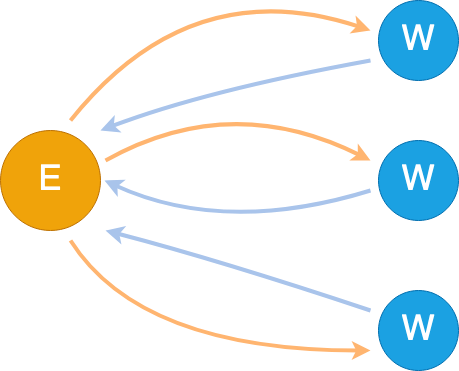
\includegraphics[scale=0.35]{img/FastFlow/Farm_graph.drawio.png}
    
    \caption{Graphical representation of the Farm employed}
\end{figure}

\subsection*{Static Chunk Size vs Dynamic Chunk Size}
For each diagonal, the length is not always a multiple of the number of nodes available. In such cases, we round up the division to the nearest integer using the standard C++ function \texttt{std::ceil}. However, this can result in the last Worker receiving fewer elements than the others, or in the worst case, some Workers might receive no elements at all and not contribute to the computation.

A possible workaround is to determine the chunk size dynamically, recalculating it each time a task is sent. The dynamic chunk size is computed as:

\[
    dynamic\_chunk\_size = \lceil {remaining\_elements\_to\_send / remaining\_workers\_with\_no\_task}\rceil
\]

Although this approach requires slightly more computation compared to static case, it ensures a more even distribution of elements. However, if the number of elements in a diagonal is smaller than the number of nodes, some nodes will still remain inactive.

Theoretically the dynamic approach seems to be better than the static method, however when comparing the two in our measurements, as Figure \ref{FF_Chunk} shows, using a dynamic chunk size proves slower. This slowdown occurs probably because the overhead of managing communication between all \texttt{Workers} outweighed the marginal decrease in elements per \texttt{Worker}. Therefore, the algorithm defaults to using static chunk sizing, with the dynamic approach available as an optional alternative through the use of the guard \texttt{DYNAMIC\_CHUNK}.

\begin{figure}[h]
    \centering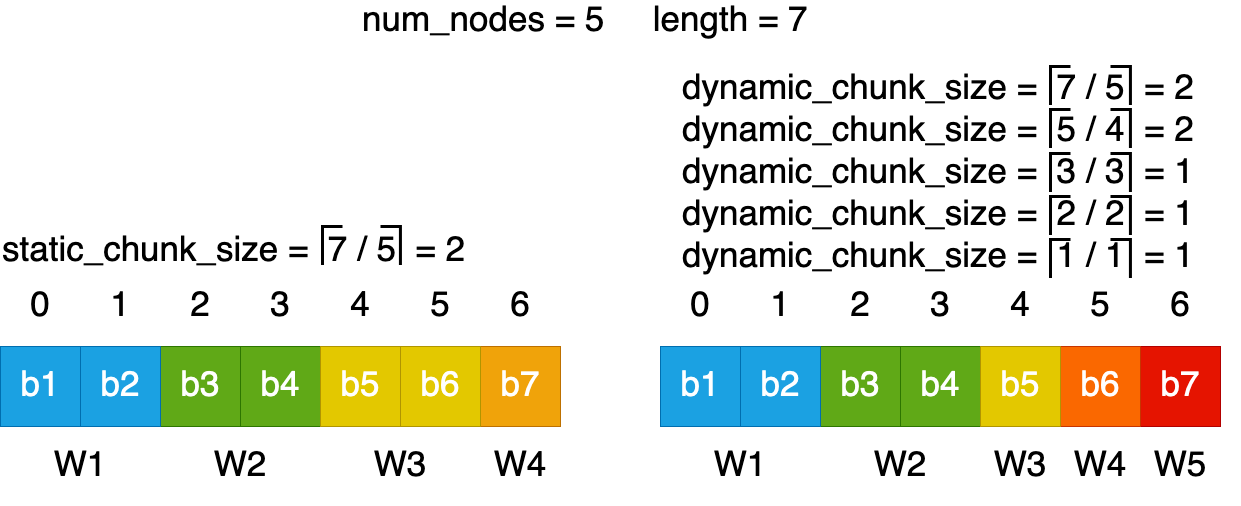
\includegraphics[scale=0.25]{img/FastFlow/Static_vs_Dynamic.drawio.png}
    
    \caption{Example of how using a dynamic chunk size compared to a static one leads to a more equal distribution among Workers}
\end{figure}

\subsection*{The DiagInfo class}
Each node needs to track the current diagonal it is processing and its length to determine which elements to compute. Instead of requiring each node to update a local copy of these values with each new task, the information is shared in the object of custom type \texttt{DiagInfo}. Only the \texttt{Emitter} has the responsibility to update before sending the task the object through the \texttt{PrepareNextDiagonal()} method and by filling the dynamic chunk size array. The \texttt{Worker}s simply read from it during their computations.

\subsection*{Farm Limitation}
Another potential parallel optimization lies in the dot product computation. Instead of calculating it element by element, the row and column vectors could be divided into segments, with each segment handled by a different thread. The partial results would then be summed to produce the final dot product. While this idea is appealing, it is impractical in our current approach. As the computation progresses, the diagonals become smaller, eventually having fewer elements than available \texttt{Worker}s. For example, the last diagonal has only one element, leaving most \texttt{Worker}s idle. Unfortunately, in \texttt{FastFlow}'s \texttt{Farm} building block, \texttt{Worker}s cannot directly communicate, so coordinating this task would require extensive communication managed by the \texttt{Emitter}, leading to inefficiencies. Another option could involve switching to a sequential approach when we encounter the first diagonal that has fewer elements than the number of workers, using a \texttt{Parallel-For} construct to distribute the workload for the dot products. However, the overhead of closing the \texttt{Farm} and initializing a new parallel construct would likely outweigh any potential benefits, making this solution inefficient. 

\subsection*{Asymptotic Complexity}
Compared to the sequential approach, the asymptotic complexity of a Wavefront computation using \texttt{FastFlow} is more efficient for computing a single diagonal, as all elements can be processed simultaneously in a single step. Assume the cost of communication between the \texttt{Emitter} and one \texttt{Worker} is a constant $\mathcal{O}(c)$ with $c > 0$, the complexity simplifies to:

\begin{itemize}
    \item \textbf{Complexity of sending tasks to each Worker =} $num\_workers \times \mathcal{O}(num\_workers \times c)$

    \item \textbf{Complexity of computing all elements of one diagonal =} $ \mathcal{O}(num\_workers \times c) + \mathcal{O}(\max{chunk\_size}) = \mathcal{O}(num\_workers \times c) + \mathcal{O}(\lceil n-1 / num\_threads \rceil)$ where $n$ is the length of the matrix.

    \item \textbf{Overall complexity = } $n-1 \times (\mathcal{O}(num\_workers \times c) + \mathcal{O}(\lceil n-1 / num\_threads \rceil) ) =\mathcal{O}((n - 1) \times num\_workers \times c) + \mathcal{O}((n-1)^{2} / num\_threads)$ where $n$ is the length of the matrix.
\end{itemize}

\subsection*{Measurements}
A \texttt{C++} implementation of the \texttt{FastFlow} approach is implemented in \textit{src\_parallel\_fastflow.cpp}. The program takes the matrix size and the number of threads as arguments. By passing $m$ and $n$, the process creates one \texttt{Emitter} and $n - 1$ \texttt{Workers} to handle a matrix of size $m$. When compiling the project using the CMake configuration files, it will generate two executables: one using static chunk sizes and the other using dynamic chunk sizes. Both versions have been tested on the \textit{``spmcluster.unipi.it''} compute cluster with various thread counts and matrix sizes. 
\par 
The speedup graph in Figure \ref{FF_Speedup} demonstrates that using more threads results in greater performance gains. However, the efficiency graph in Figure \ref{FF_Efficiency} reveals that as the number of threads increases, efficiency diminishes, indicating that the overhead associated with managing additional threads becomes more and more large. This suggests to take into account the computational cost of coordinating a larger number of threads when computing the Wavefront pattern in a shared memory setting.

\begin{figure}[h!]
    \centering
    % First row: Two images adjacent
    \begin{minipage}[t]{0.49\textwidth}
        \centering
        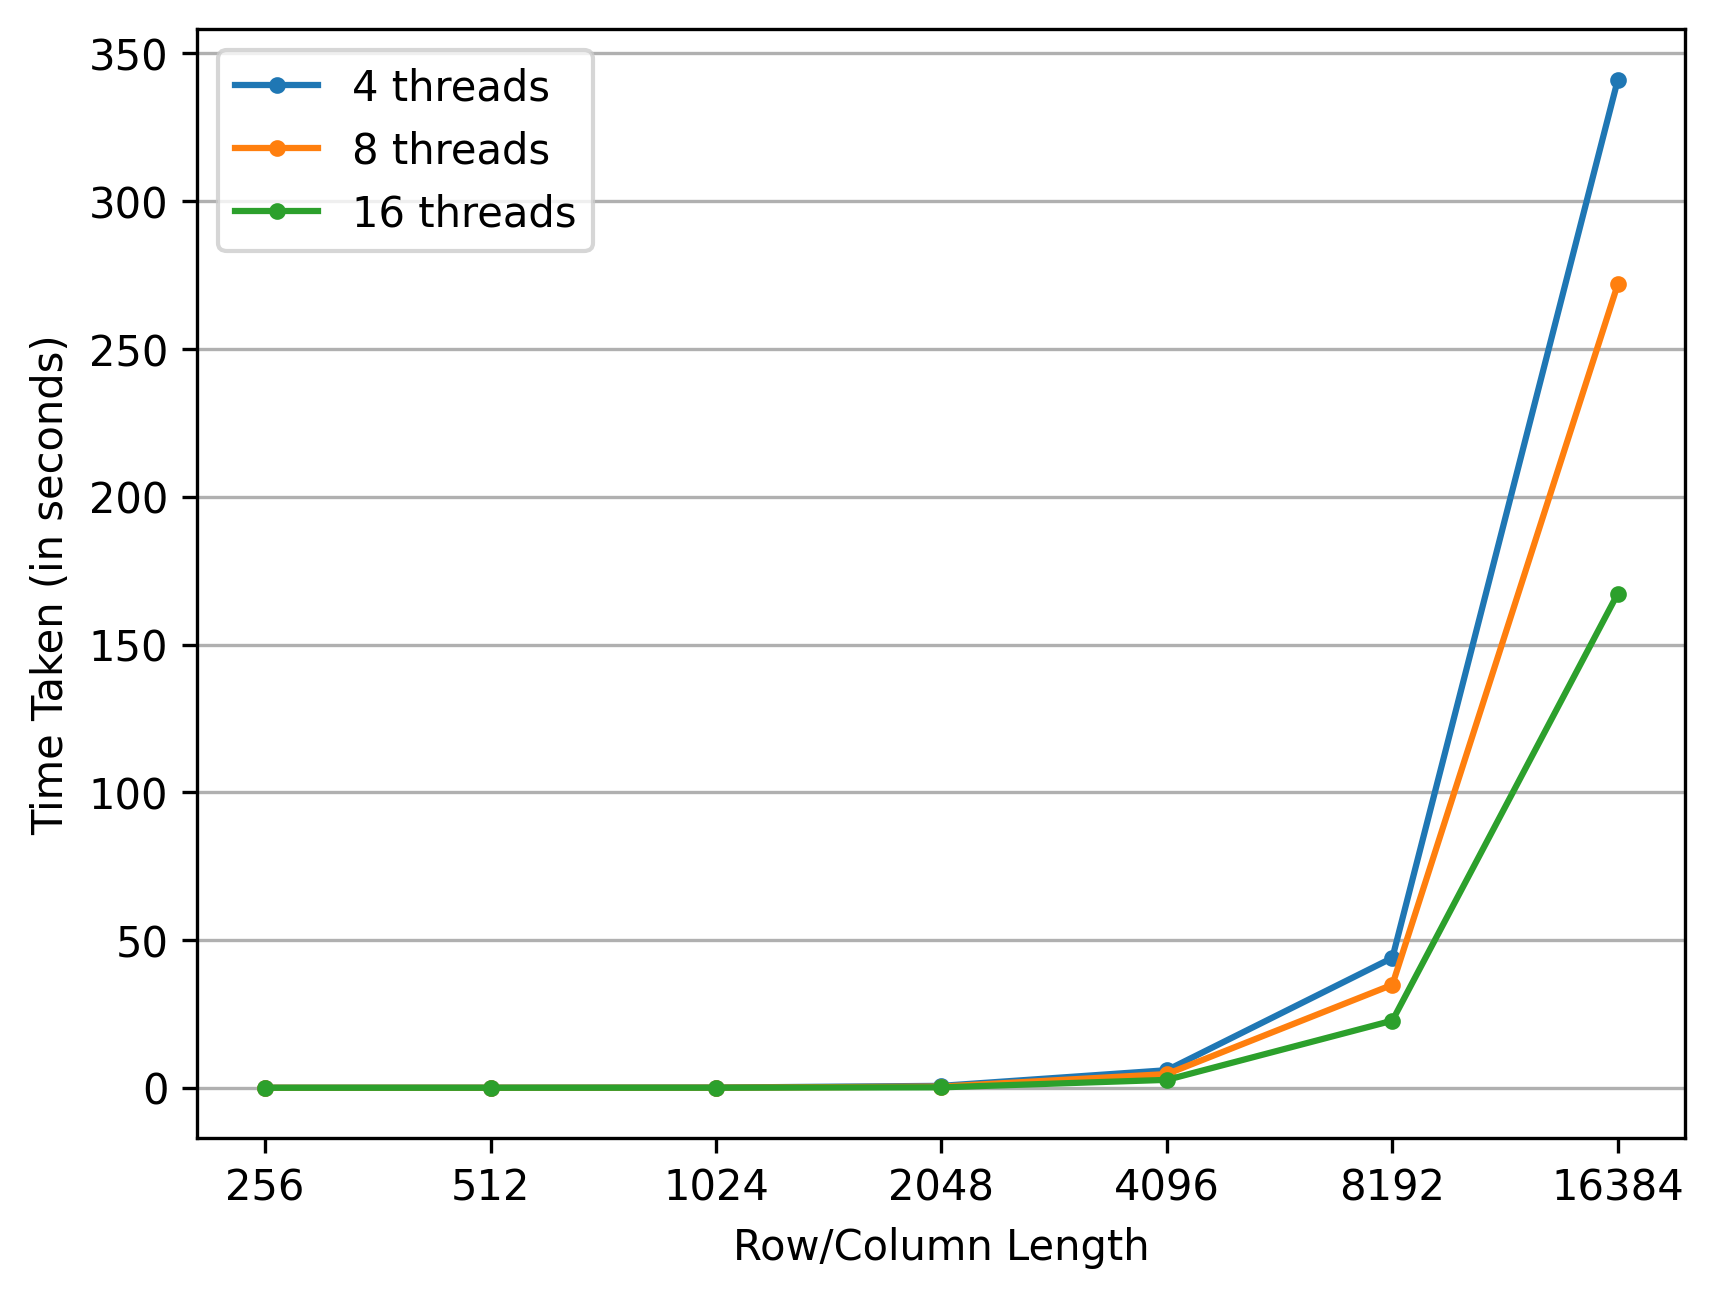
\includegraphics[width=\textwidth]{img/FastFlow/ff_static_graph.png}
        \caption{Strong scaling comparison}
        \label{FF_Strong_scaling}
    \end{minipage}
    \hfill
    \begin{minipage}[t]{0.49\textwidth}
        \centering
        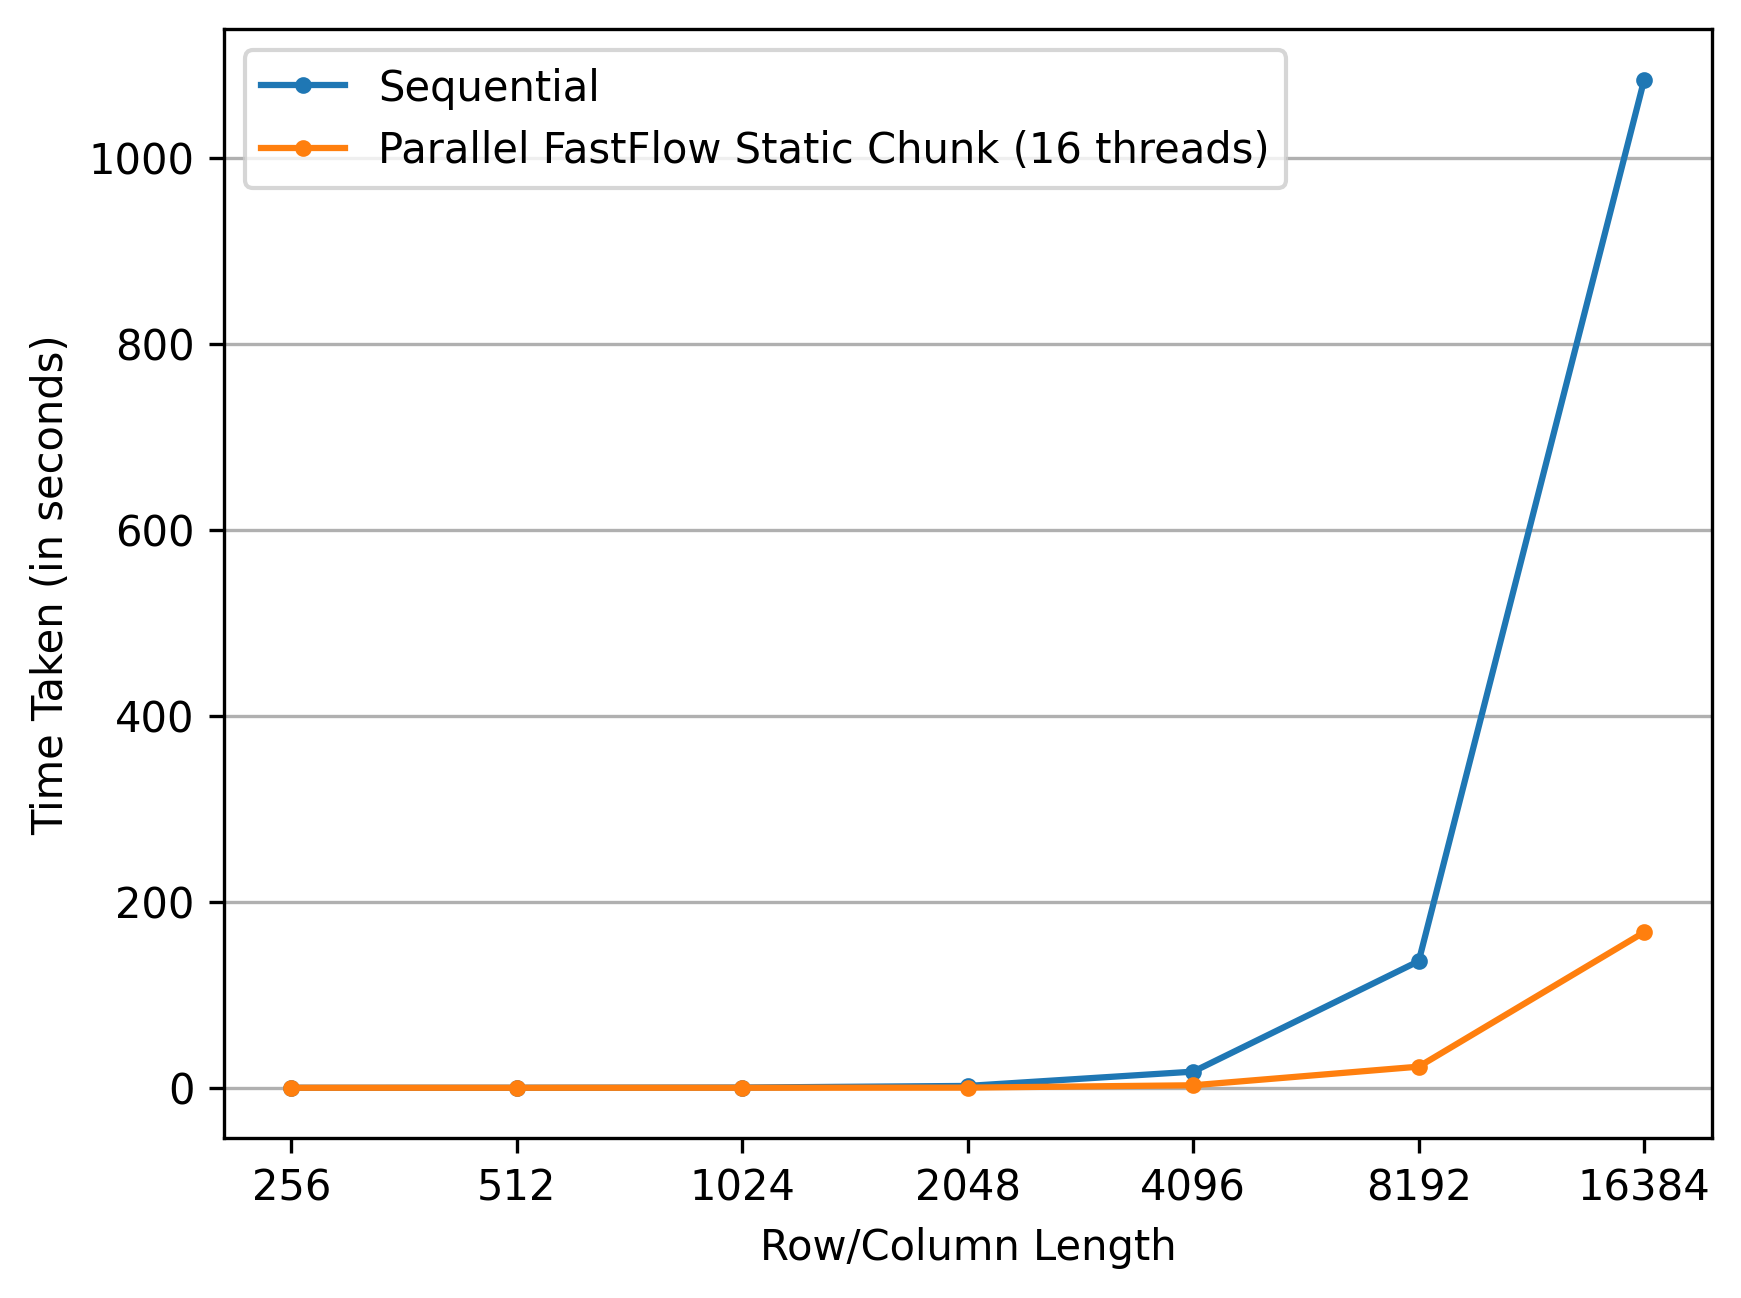
\includegraphics[width=\textwidth]{img/FastFlow/ff_sequential_vs_fastflow.png}
        \caption{Comparison between sequential and FastFlow}
        \label{FF_Sequential_vs_FastFlow}
    \end{minipage}
    
    % First row: Two images adjacent
    \begin{minipage}[t]{0.49\textwidth}
        \centering
        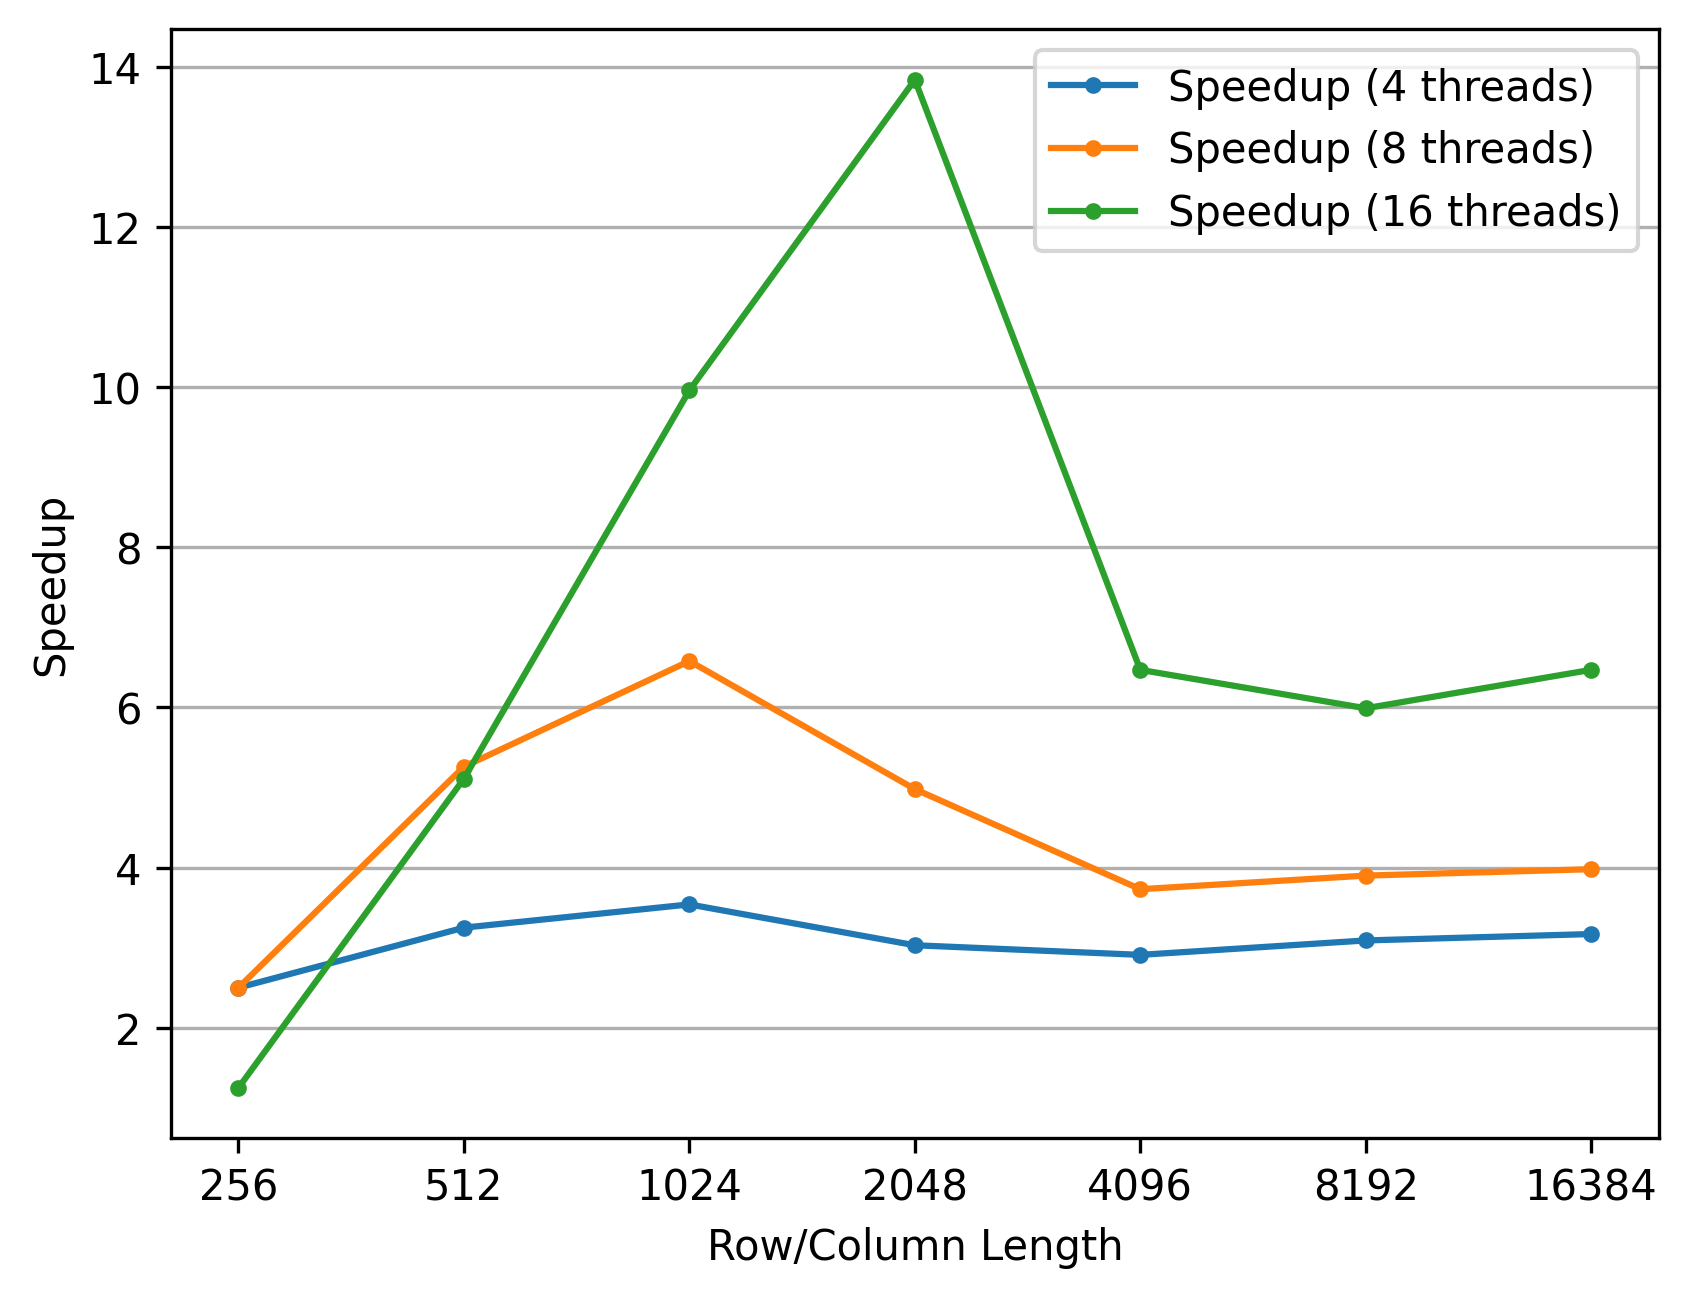
\includegraphics[width=\textwidth]{img/FastFlow/ff_speedup.png}
        \caption{Speedup comparison in FastFlow}
        \label{FF_Speedup}
    \end{minipage}
    \hfill
    \begin{minipage}[t]{0.49\textwidth}
        \centering
        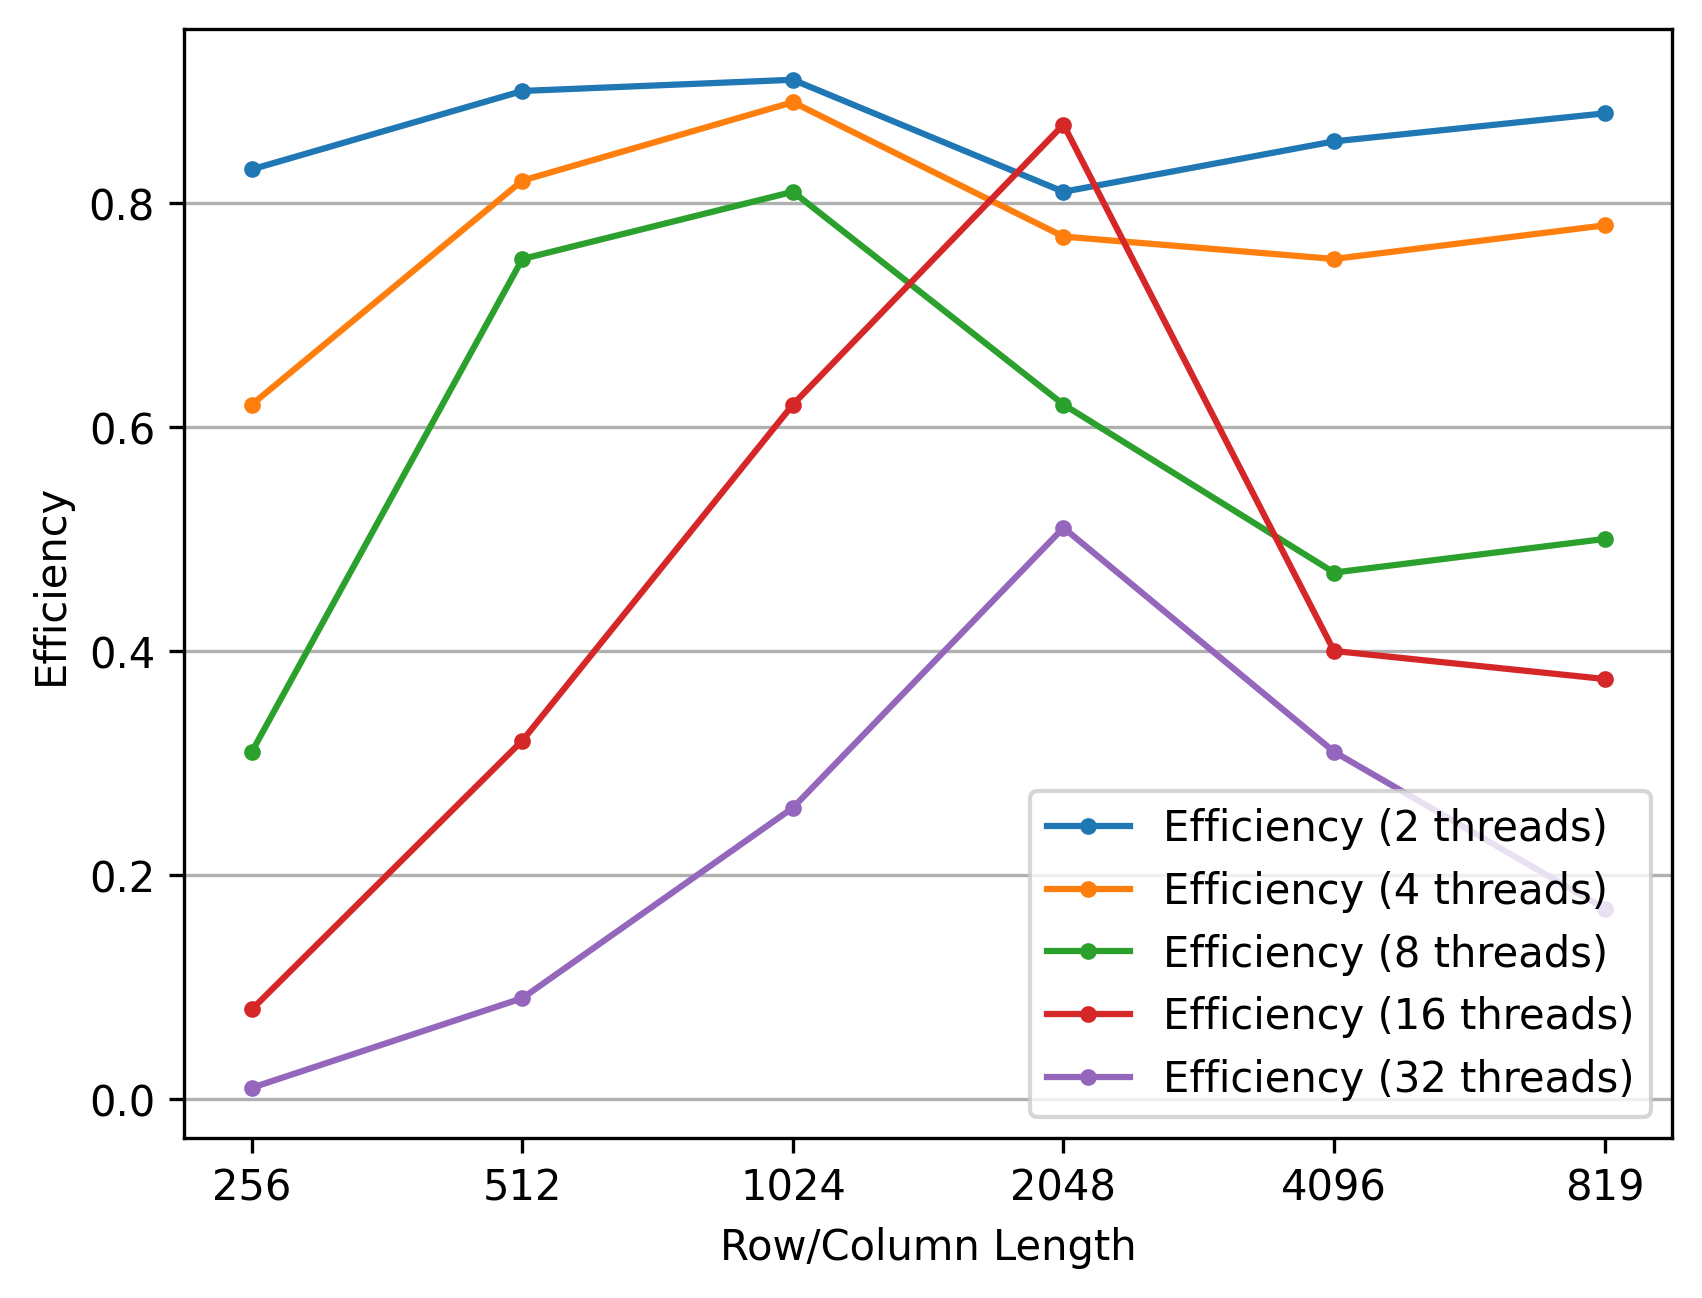
\includegraphics[width=\textwidth]{img/FastFlow/ff_efficiency.png}
        \caption{Efficiency comparison in FastFlow}
        \label{FF_Efficiency}

    \end{minipage}
    \begin{minipage}[t]{0.65\textwidth}
        \centering
        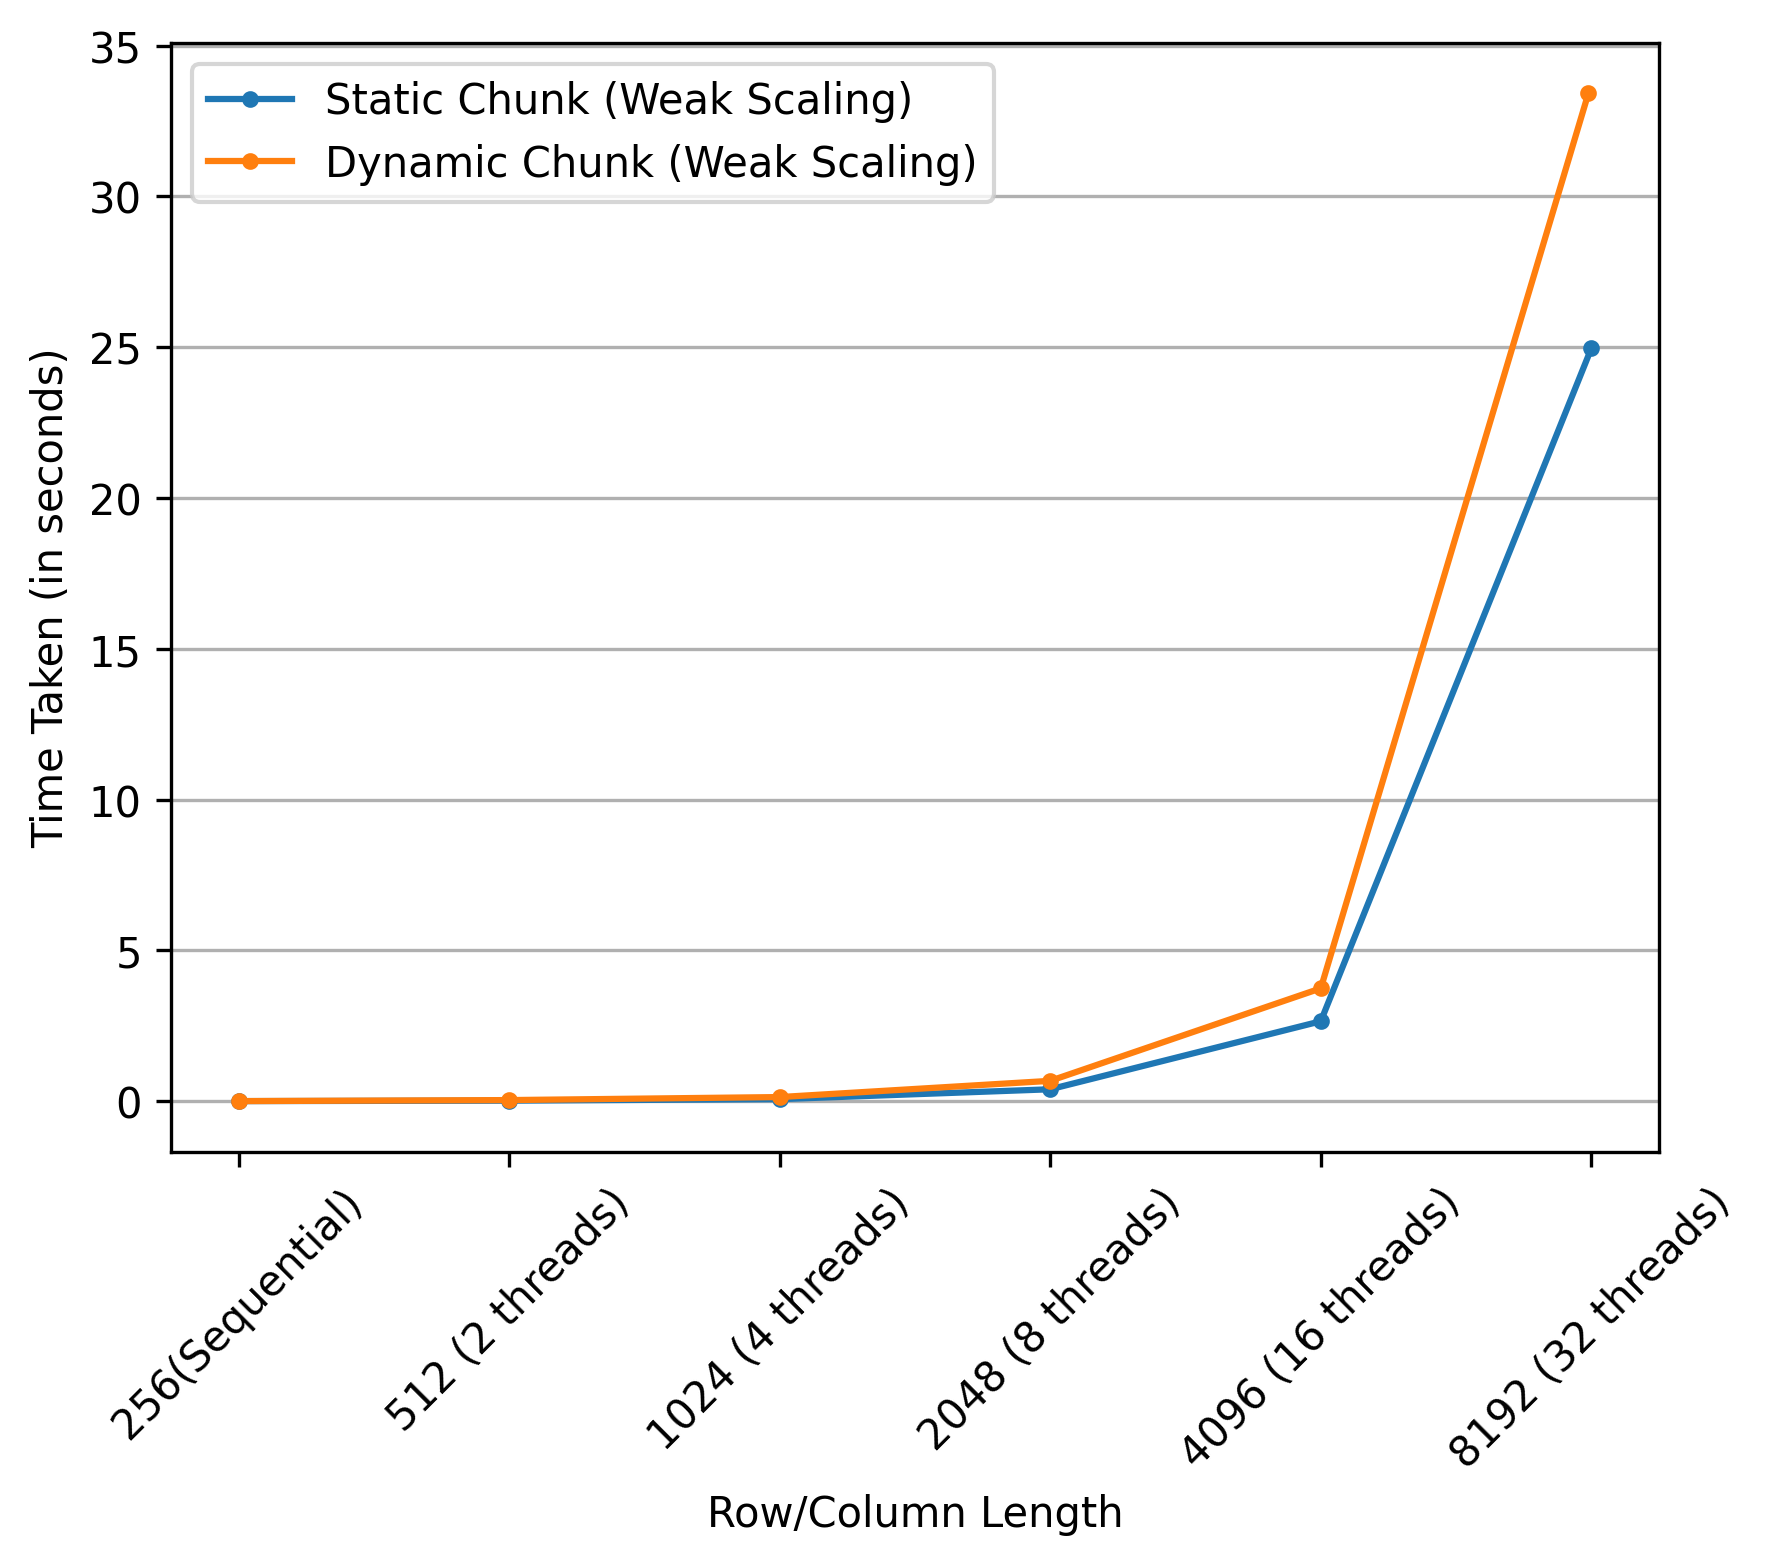
\includegraphics[width=\textwidth]{img/FastFlow/ff_static_vs_dynamic.png}
        \caption{Weak scaling of chunck approaches}
        \label{FF_Chunk}
    \end{minipage}
\end{figure}